% Пример заготовки для презентации с использованием класса Beamer LaTeX.
% Версия от 09 ноября 2018 года.
\documentclass[12pt,a4paper,mathserif]{beamer}
\usepackage[utf8x]{inputenc}
\usepackage{ucs}
\usepackage[T2A]{fontenc}
\usepackage[english,russian]{babel}
\usepackage{amsmath}
\usepackage{amsfonts}
\usepackage{amssymb}
\usepackage{mathtext}
\usepackage{graphicx}
\usepackage{enumerate}
\usepackage{multirow}
\usepackage{ragged2e}
\justifying
\renewcommand{\raggedright}{\leftskip=0pt \rightskip=0pt plus 0cm}
\setbeamertemplate{caption}[numbered]

\usetheme {Madrid}
\usecolortheme [RGB={85, 107, 47}]{structure} %Dark Olive Green

\author{Лаптев Александр}
\title{Создание информационной системы}

\begin{document}
\begin{frame}
\maketitle
\end{frame}

\begin{frame}{Создание информационной системы}
    \setlength{\parindent}{0.5cm}
    Цель: в заключительном задании по курсу требовалось создать информационную систему для предприятия, которое занимается производством цитрусовых и их последующей переработкой.
    
    Требования к ИС:
    \begin{enumerate}
        \item Наличие подсистем;
        
        \item Наличие всех видов справочников;
        
        \item Наличие документов (не менее 5 типов);
        
        \item Наличие регистров (не менее 5 типов);
        
        \item Наличие отчетов (не менее 10 видов).
    \end{enumerate}
\end{frame}

\begin{frame}{Разбиение ИС на подсистемы}
    \setlength{\parindent}{0.5cm}
    В результате создания состава подсистем ИС были выделены следующие функциональные части:
    
    \begin{enumerate}
        \item Бухгалтерия
        
        \item Учет Сырья
        
        \item Учет Готовой Продукции
        
        \item Продажи
        
        \item Предприятие
    \end{enumerate}
\end{frame}

\begin{frame}{Создание справочников}
    \begin{figure}
        \centering
        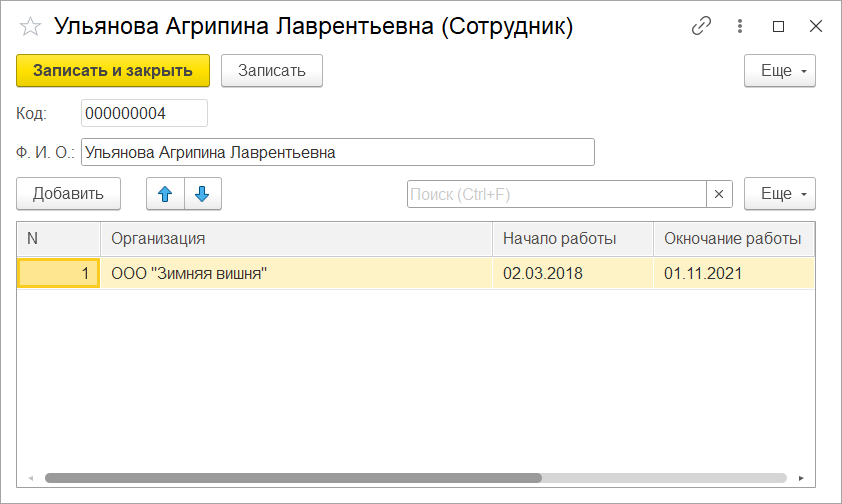
\includegraphics[scale=0.6]{worker.png}
        \caption{Справочник с табличной частью}
        \label{fig:table}
    \end{figure}
\end{frame}

\begin{frame}{Создание справочников}
    \begin{figure}
        \centering
        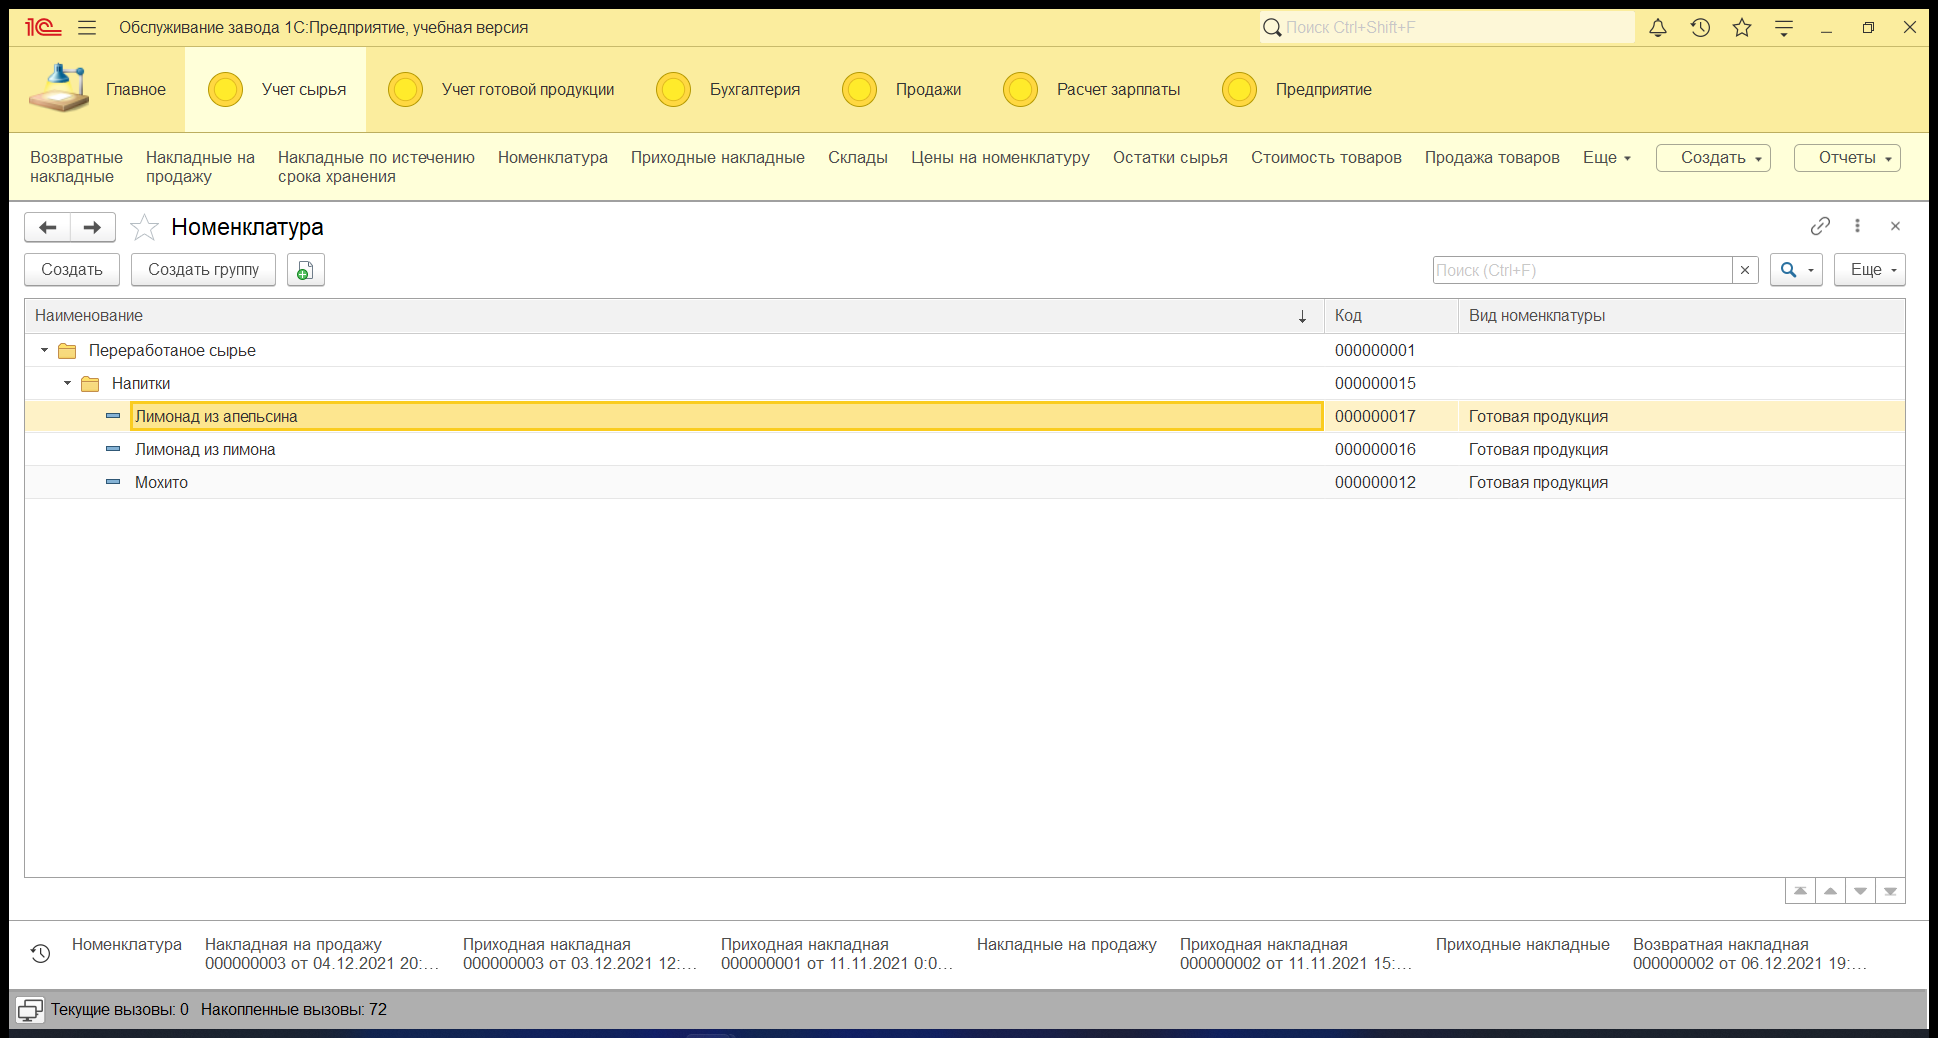
\includegraphics[scale=0.25]{nomenclature.png}
        \caption{Иерархический справочник}
        \label{fig:nomenclature}
    \end{figure}
\end{frame}

\begin{frame}{Создание документов}
    \begin{figure}
        \centering
        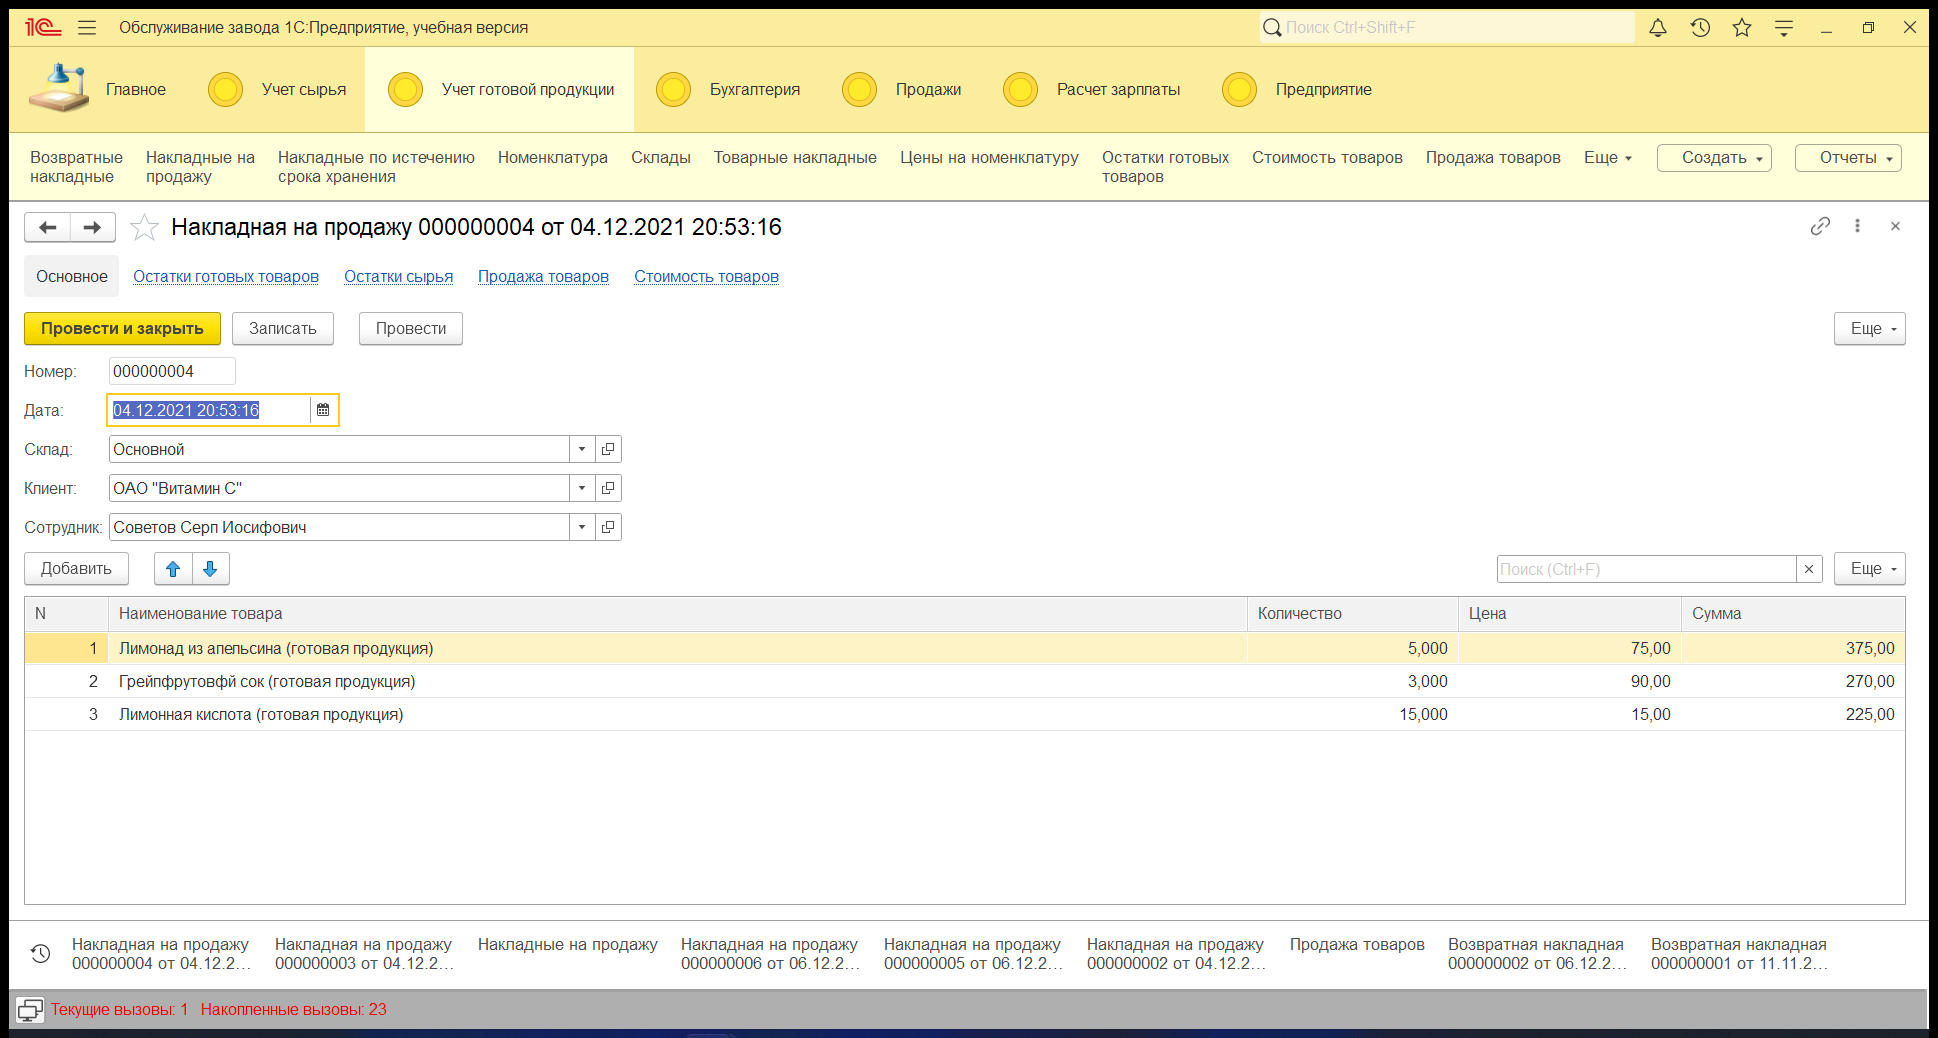
\includegraphics[scale=0.25]{document.png}
        \caption{Пример документа}
        \label{fig:document}
    \end{figure}
\end{frame}

\begin{frame}{Создание регистров}
    \begin{figure}
        \centering
        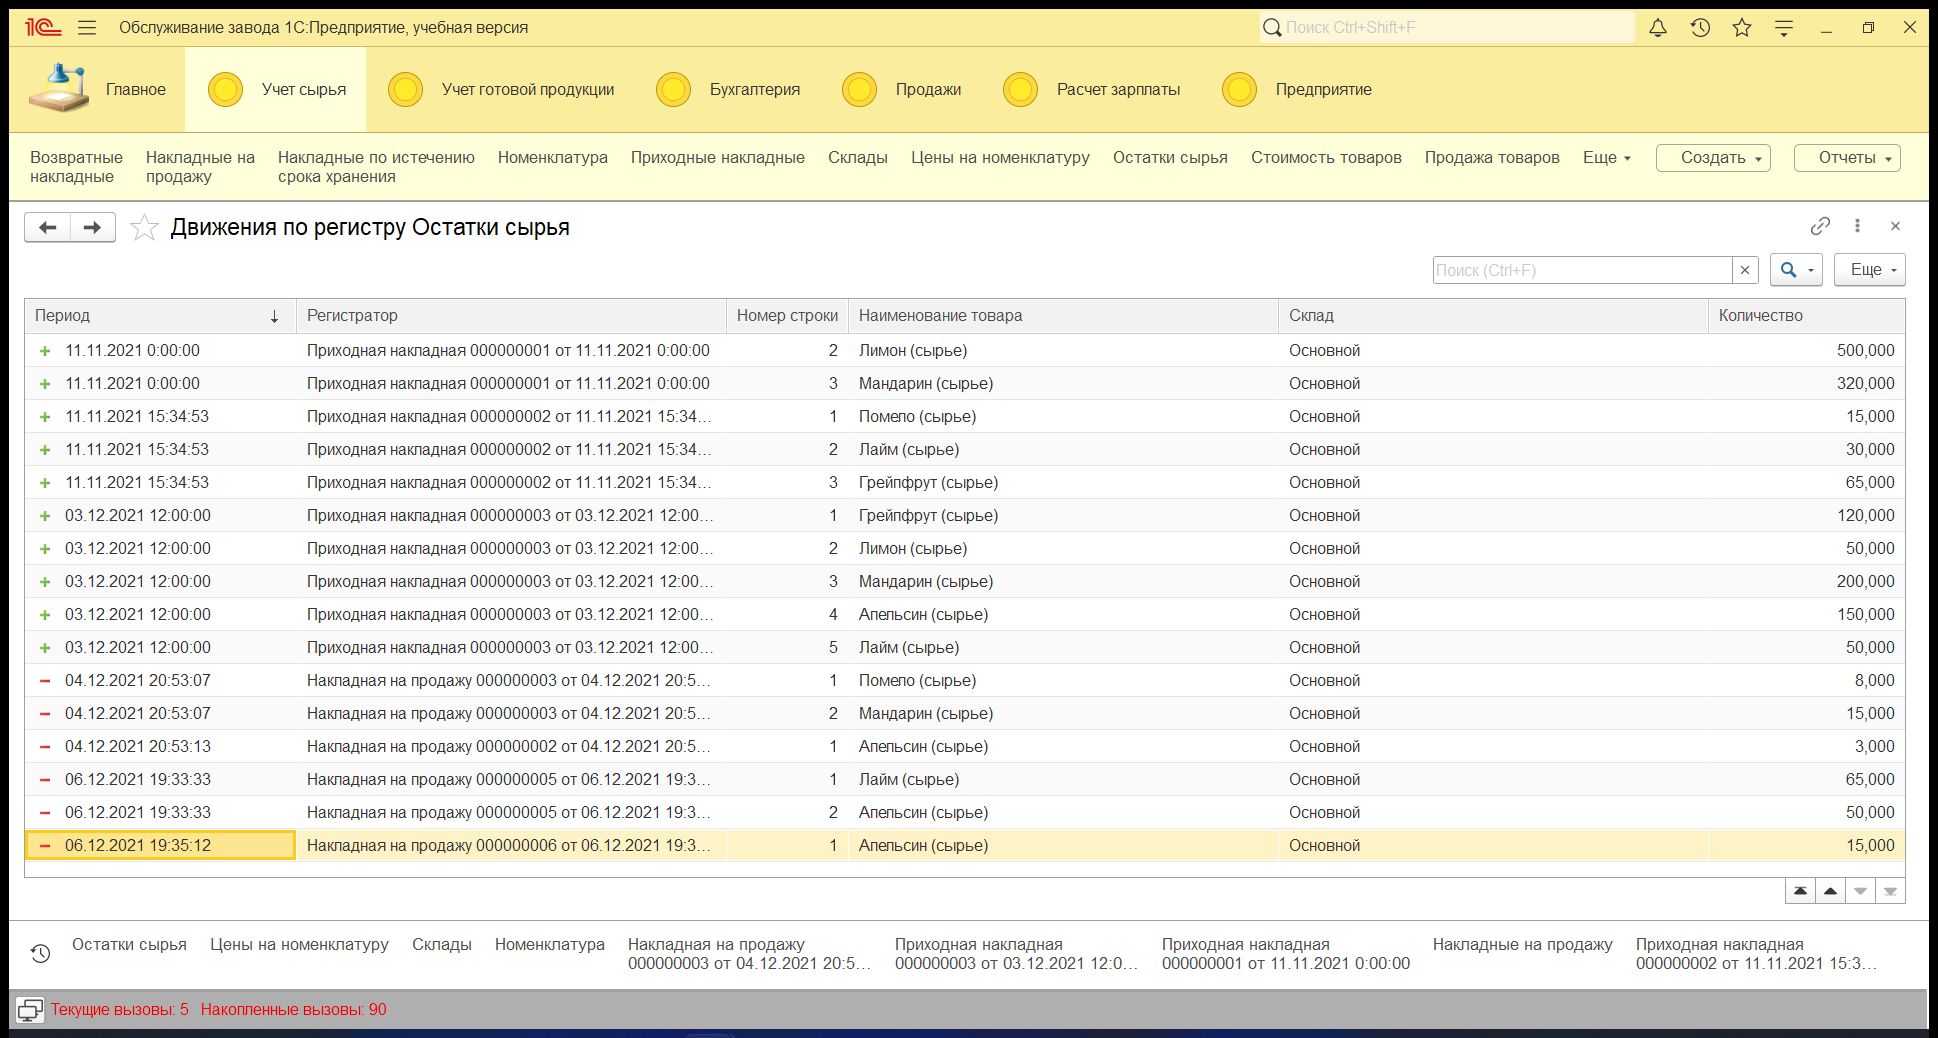
\includegraphics[scale=0.25]{accumulation.png}
        \caption{Регистр накопления}
        \label{fig:accumulation}
    \end{figure}
\end{frame}

\begin{frame}{Создание регистров}
    \begin{figure}
        \centering
        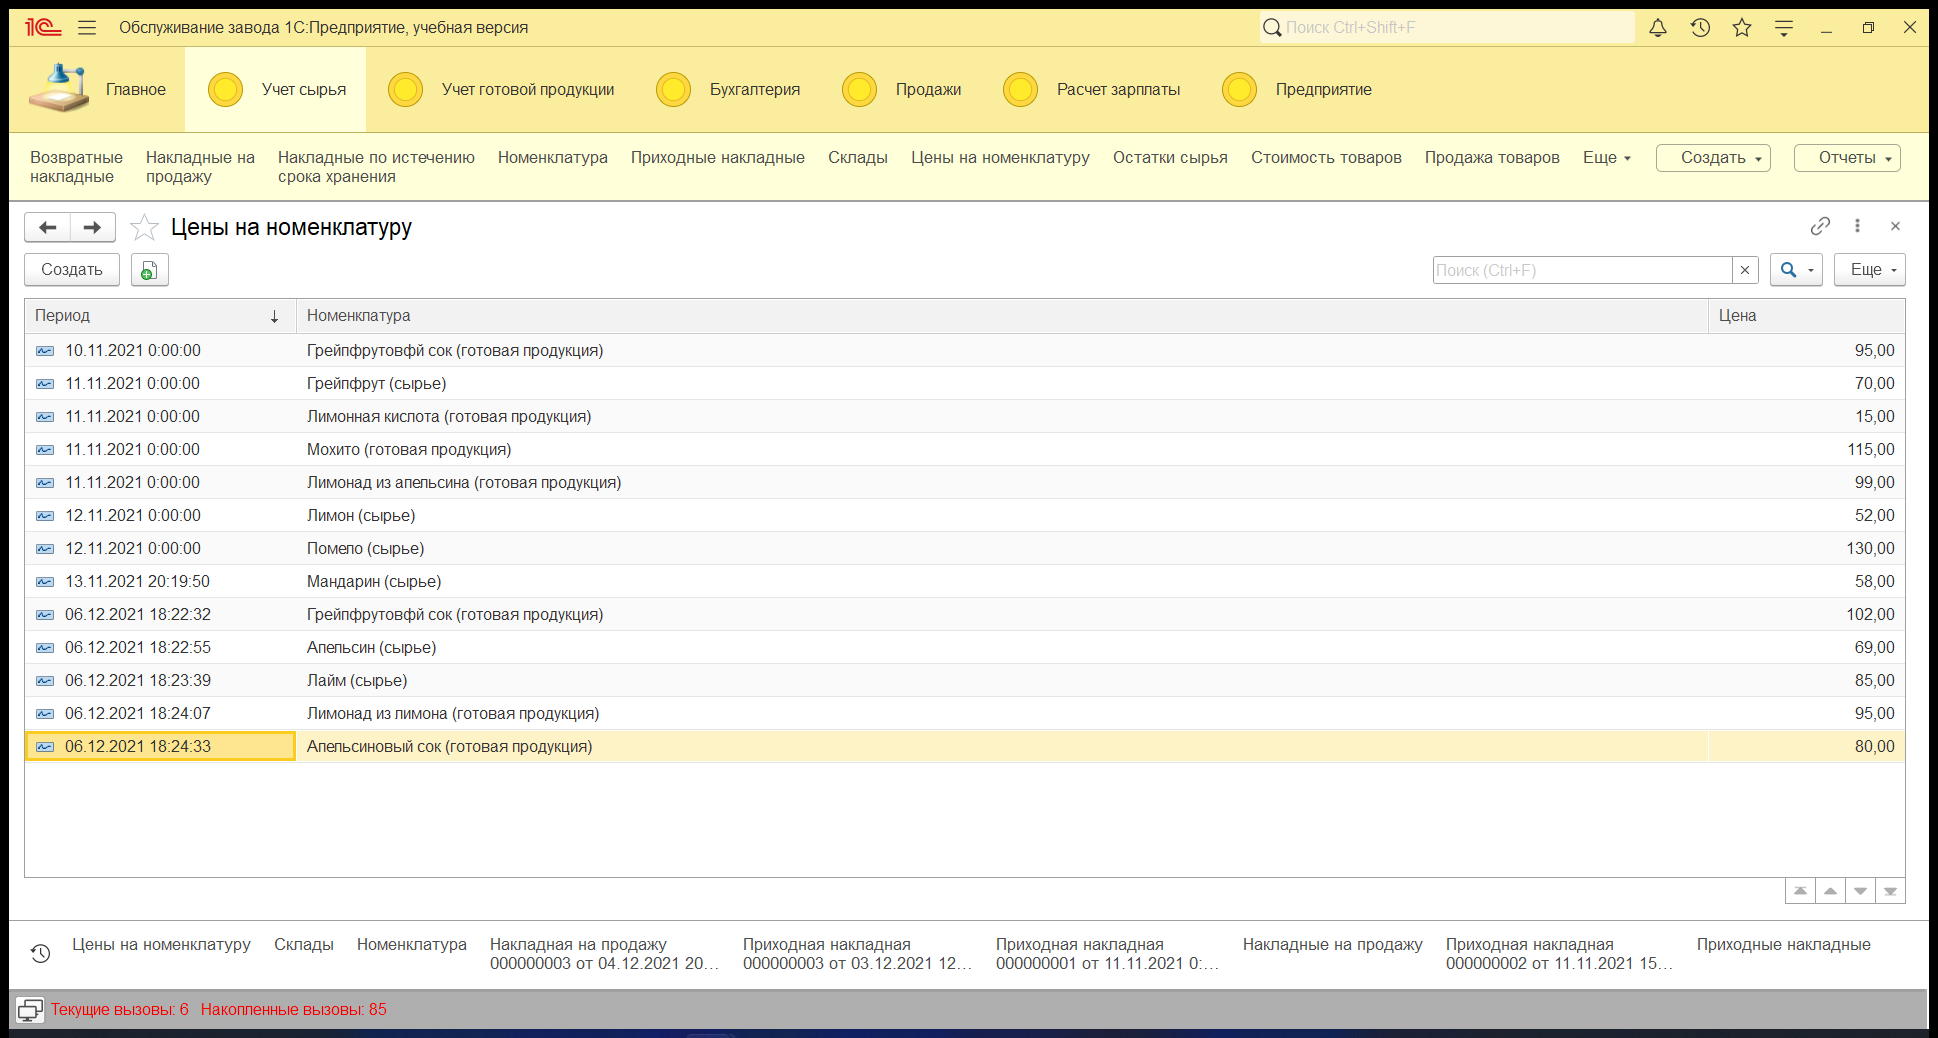
\includegraphics[scale=0.25]{information.png}
        \caption{Регистр сведений}
        \label{fig:information}
    \end{figure}
\end{frame}

\begin{frame}{Создание отчетов}
    \begin{figure}
        \centering
        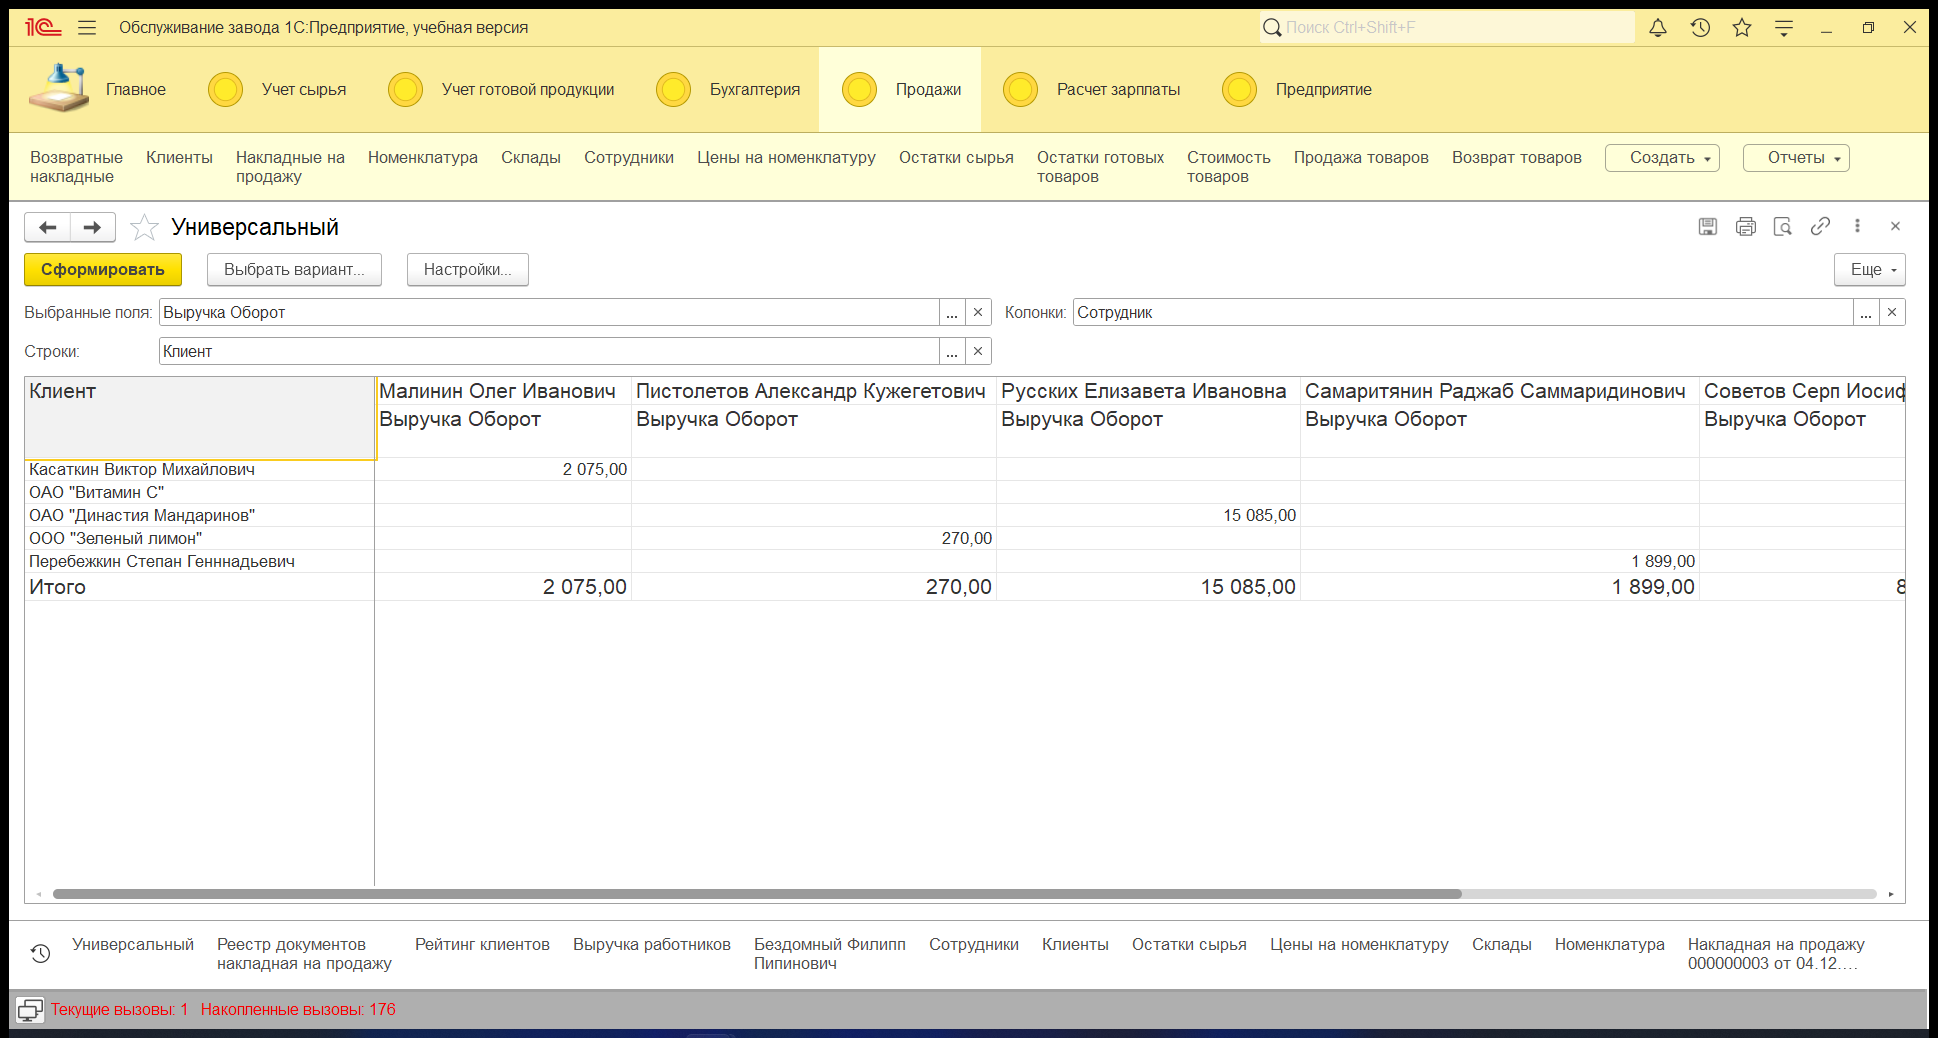
\includegraphics[scale=0.25]{universal.png}
        \caption{Универсальный отчет}
        \label{fig:universal}
    \end{figure}
\end{frame}

\begin{frame}{Создание отчетов}
    \begin{figure}
        \centering
        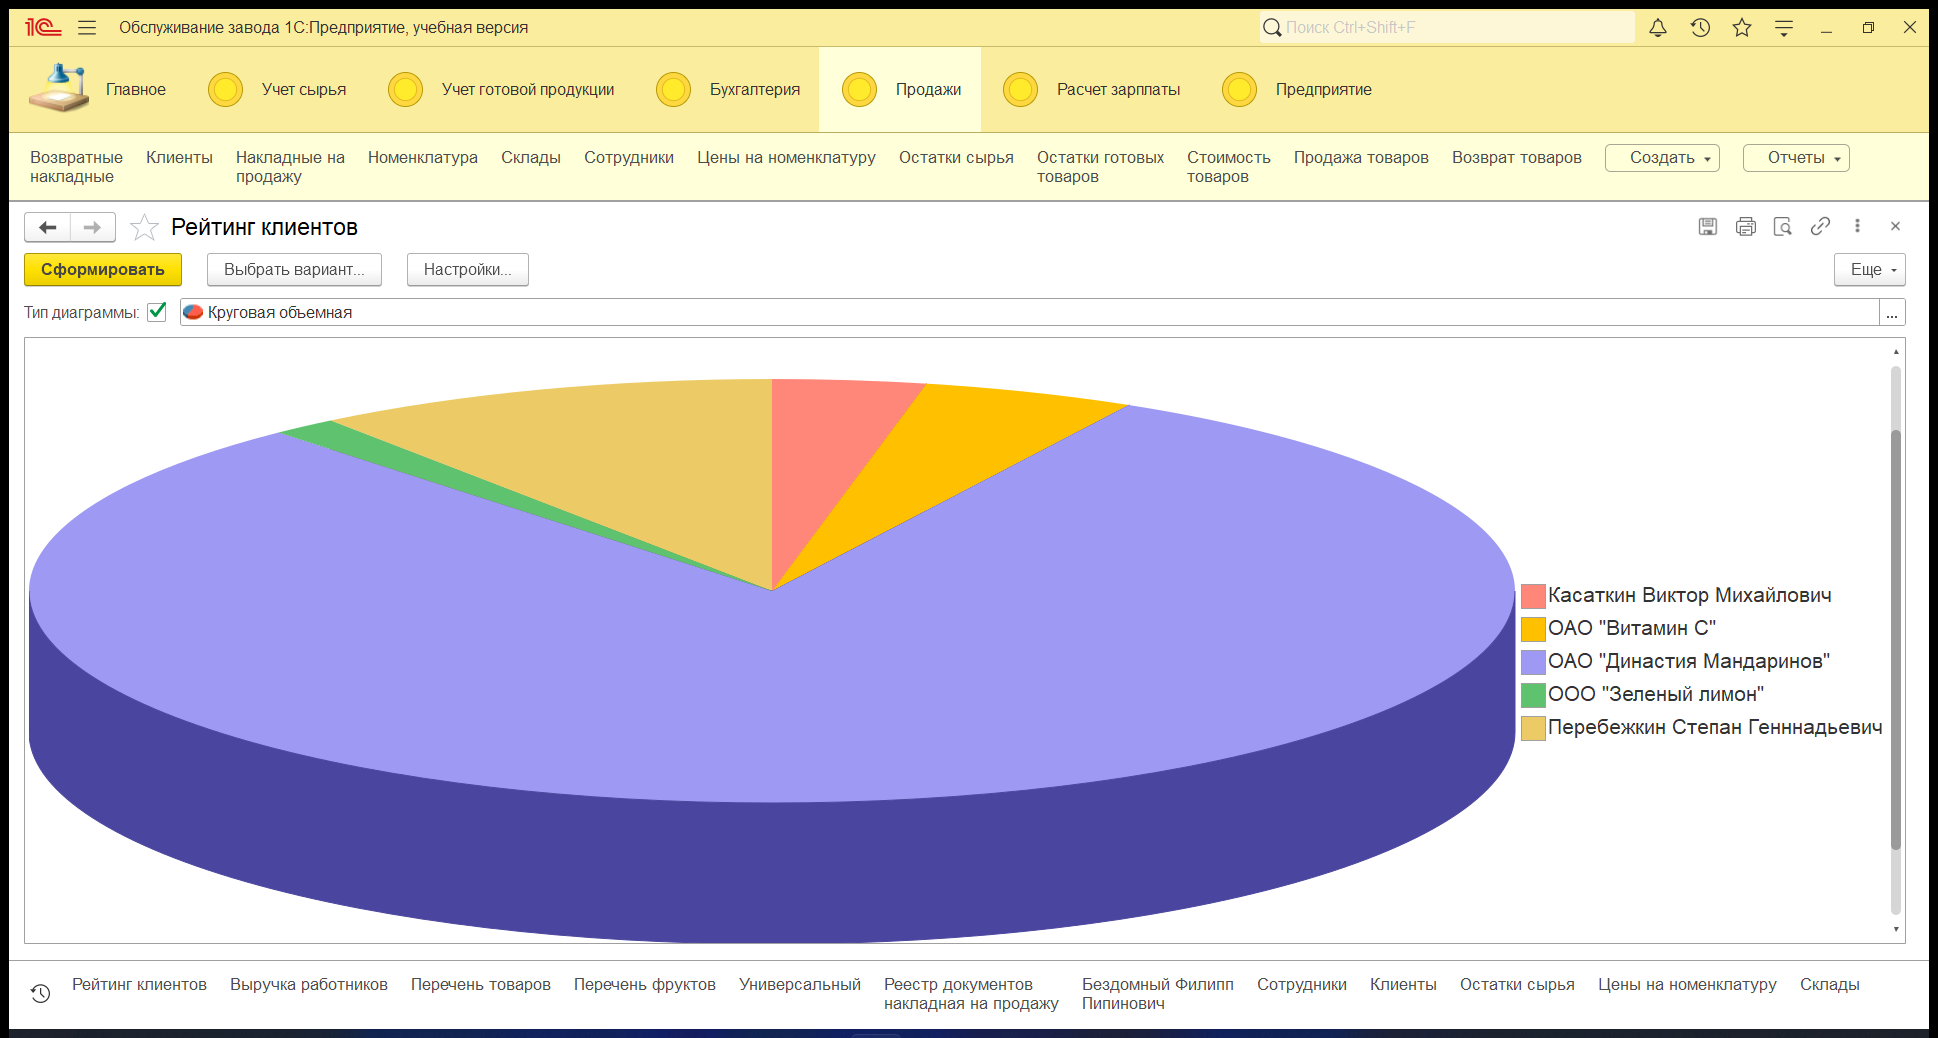
\includegraphics[scale=0.25]{client.png}
        \caption{Отчет с применением диаграммы}
        \label{fig:client}
    \end{figure}
\end{frame}

\end{document}
